\section{نبود سیاه‌چاله}
در یک شبکه سیاه‌چاله‌ها
\lf{Blackhole}
عناصری در شبکه هستند که وظیفه ارسال بسته‌ها را دارند
(مثلا سوییچ‌ یا روتر)
ولی برخی از بسته‌ها را پس از دریافت به جایی ارسال نمی‌کنند و در واقع مانند سیاه‌چاله این بسته‌ها در آن‌ها گم می‌شوند
\cite{network-abstractions}.
در یک شبکه که مکان‌های ورودی و خروجی مشخص دارد عدم وجود سیاه‌چاله در شبکه را می‌توان معادل این ويژگی که همه‌ی بسته‌های ورودی به شبکه از آن خارج شوند دانست.
\begin{figure}
    \centering
    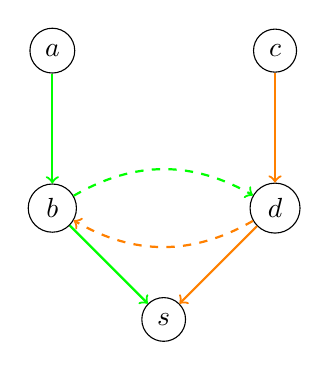
\begin{tikzpicture}[
            node distance={20mm},
            main/.style = {draw, circle},
            s/.style = {->,thick},
            d/.style = {->,thick,dashed} ]
        \node[main] (s) {$s$};
        \node[main] (b) [above left of=s] {$b$};
        \node[main] (a) [above of=b] {$a$};
        \node[main] (d) [above right of=s] {$d$};
        \node[main] (c) [above of=d] {$c$};
        \draw[thick,green,->] (a) -- (b);
        \draw[thick,green,->] (b) -- (s);
        \draw[thick,green,->,dashed] (b) edge[bend left] (d);
        \draw[thick,orange,->] (c) -- (d);
        \draw[thick,orange,->] (d) -- (s);
        \draw[thick,orange,->,dashed] (d) edge[bend left] (b);
    \end{tikzpicture}
    \caption{ }
    \label{fig:blackhole}
\end{figure}
به عنوان مثال شبکه‌ی موجود در شکل
\ref{fig:blackhole}
را در نظر بگیرید.
فرض کنید که در این شبکه
$a,c$
ورودی‌های شبکه و
$s$
خروجی شبکه باشد.
در این شبکه دو به روز رسانی برای جایگزینی
مسیر
$ds$
با
$db$
و مسیر
$bs$
با
$bd$
انجام می‌شود.
در این شبکه در حالت ابتدایی و پس از انجام یکی از به روز‌رسانی‌ها ورودی‌ها به خروجی مسیر وجود دارد اما اگر هر دوی این به روز رسانی‌ها انجام شوند دیگر
$s$
قابل دسترسی نیست و عملا بسته‌های ورودی به شبکه به خروجی نمی‌رسند.
این شبکه را می‌توانیم به فرم زیر در نت‌کت پویا توصیف کنیم:
\begin{equation*}
    \begin{aligned}[c]
        P   & = p!1                             \\
        Q   & = q!1                             \\
        N   & = F \oplus p?1;N_p \oplus q?1;N_q \\
        N_p & = F \oplus q?1;F_{pq}             \\
        N_q & = F \oplus p?1;F_{pq}
    \end{aligned}
    \qquad\qquad
    \begin{aligned}[c]
        F           & = a\ra s \oplus c\ra s            \\
        F_{pq}      & = a\ra b \oplus c\ra d            \\
        SDN         & = \delta_{\mathcal{L}} (N
        \parallel P \parallel Q)                \\
        \mathcal{L} & = \s{p!1,p?1,q?1,q?1}
    \end{aligned}
\end{equation*}
در ادامه فرض کنید که 
$\mc{M}$
مدل علّی این شبکه باشد.
در این مدل تابع متغیر
$PV$
را به صورت زیر تعریف می‌کنیم:
\begin{align*}
    \f{PV} & = \exists c \in \mathcal{F}(ES(\vec v)),
    \exists e \in c. l(e) =  \alpha\cdot\pi \wedge \pi(sw) \neq s
\end{align*}
در تعریف این تابع رفتار نا امن وجود یک پیکربندی شامل رویدادی با برچسب از نوع 
$\alpha \cdot \pi$
یا به عبارت دیگر رویدادی از نوع ارسال بسته است که سوییچ مقصد ارسال آن سوییچ 
$s$
نباشد.
همانند مثال مربوط نبود دور در شبکه، در این مثال هم با توجه به ترتیب اجرای به روز رسانی‌ها دو رویداد برای هر یک از عملیات‌های 
$rcfg(p!1,p?1)$
،$rcfg(q!1,q?1)$
و
$a\ra b,a c\ra d$
وجود دارد. 
بنابراین فرض کنید که رویدادهای
$p_i,q_i,ab_i,cd_i$
به ازای 
$i=1,2$
در ساختمان رویداد این مدل وجود داشته باشند و برچسب‌گذاری آن‌ها به صورت زیر باشد:
\begin{align*}
    l(p_1) & = rcfg(p!1,p?1) \\
    l(p_2) & = rcfg(p!1,p?1) \\
    l(q_1) & = rcfg(q!1,q?1) \\
    l(q_2) & = rcfg(q!1,q?1) \\
    l(ab_1) & = a \ra b \\
    l(ab_2) & = a \ra b \\
    l(cd_1) & = c \ra d \\
    l(cd_2) & = c \ra d \\
\end{align*}
\begin{figure}
    \centering
    \begin{tikzpicture}
        \crd{0}{0}{$\emptyset$}
        \crd[left]{-2}{1}{$\s{p_1}$}
        \crd[left]{-2}{2}{$\s{p_1,q_1}$}
        \crd[above]{-1}{3}{$\s{p_1,q_1,ab_1}$}
        \crd[left]{-3}{3}{$\s{p_1,q_1,cd_1}$}
        \crd[right]{2}{1}{$\s{q_2}$}
        \crd[right]{2}{2}{$\s{p_2,q_2}$}
        \crd[above]{1}{3}{$\s{p_2,q_2,ab_2}$}
        \crd[right]{3}{3}{$\s{p_2,q_2,cd_2}$}
        \draw [ultra thick] (-2,1) -- (-2,2);
        \draw [ultra thick] (-2,2) -- (-1,3);
        \draw [ultra thick] (-2,2) -- (-3,3);
        \draw [ultra thick] (0,0) -- (2,1);
        \draw [ultra thick] (0,0) -- (-2,1);
        \draw [ultra thick] (2,1) -- (2,2);
        \draw [ultra thick] (2,2) -- (1,3);
        \draw [ultra thick] (2,2) -- (3,3);
    \end{tikzpicture}
    \caption{}
    \label{fig:blackhole:es}
\end{figure}
پیکربندی‌هایی از این ساختمان رویداد که شامل رویدادی با برچسب 
$a \ra b$
یا 
$c \ra d$
باشند نقض شدن ویژگی نبود سیاه‌چاله را نشان می‌دهند.
بنابراین تابع متغیر
$PV$
را به فرم زیر توصیف می کنیم:
\begin{align*}
    \f{PV} & = \exists c \in \mathcal{F}(ES(\vec v)),
    \exists e \in c. l(e) =  \alpha\cdot\pi \wedge \pi(sw) \neq s
\end{align*}
در این مدل هم همانند مثال نبود دور در شبکه عدم وجود تعارض بین رویداد‌های 
$p_1$
و
$q_1$
را می‌توان به عنوان علت واقعی نقض شدن ویژگی در نظر گرفت.
برای این منظور از شاهد
$(C_{p_2,q_2},\T,\T)$
استفاده می‌کنیم.
واضح است که اگر مقدار هر دو متغیر
$C_{p_1,q_1}$
و
$C_{p_2,q_2}$
را برابر غلط قرار دهیم آنگاه هیچ یک از پیکر‌بندی‌های 
$\s{p_1,q_1,cd_1},\s{p_1,q_1,ab_1},\s{p_2,q_2,ab_2},\s{p_2,q_2,cd_2}$
دیگر عضوی از پیکربندی‌های 
$ES(\vec v)$
نیستند.
از طرفی در شرایطی که 
$C_{p_1,q_1}$
مقدار درست داشته باشد آنگاه پیکربندی‌های
$\s{p_1,q_1,ab_1},\s{p_1,q_1,cd_1}$
عضو
$ES(\vec v)$
هستند و مقدار متغیر
$C_{p_2,q_2}$
تاثیری روی این مساله ندارد بنابراین در نهایت می‌توان نتیجه گرفت که 
$C_{p_1,q_1} = \F$
علت واقعی نقض ویژگی است.